\documentclass{beamer}
\usetheme{Montpellier}
\usecolortheme{beaver}

\title{Rust Remote.Access.Trojan}
\author{Antoine MARTIN, Wesley EDE, Amad MOHAMMAD, Denis REMACLE}

\begin{document}

  \begin{frame}
 \maketitle
  \end{frame}

\begin{frame}{Sommaire}
    \tableofcontents
\end{frame}

\section{Qu'est-ce qu'un Remote.Access.Trojan ?}
  \begin{frame}{Qu'est-ce qu'un Remote.Access.Trojan ?}
  \begin{itemize}
	\item Un malware qui permet de prendre controle à distance et exécuter des commandes sur un poste infecté.
	\item Exemple notable : DarkComet, NanoCore
  \end{itemize}
  \end{frame}

  \begin{frame}{Qu'est-ce qu'un Remote.Access.Trojan ?}
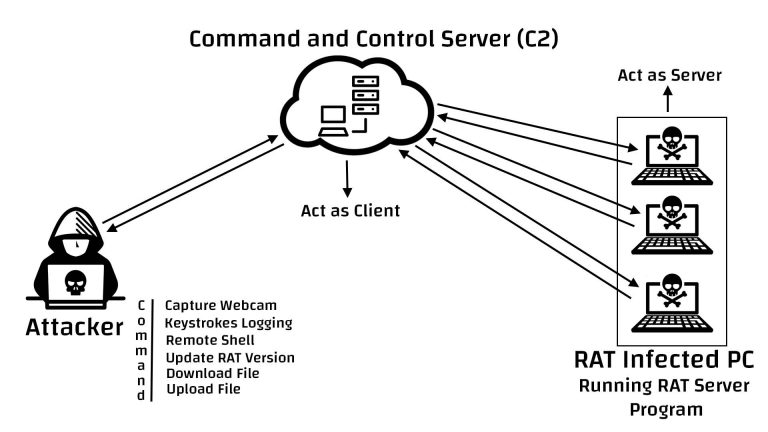
\includegraphics[scale=.4]{Schema.jpg}
  \end{frame}

\section{Et pourquoi on en code un !}
  \begin{frame}{Et pourquoi on en code un !}
  \begin{itemize}
	\item Un challenge stimulant
	\item Une occasion d'apprendre un langage dont l'importance ne fait que croitre
  \end{itemize}
  \end{frame}

\section{Comment fonctionne-t-il en somme ?}
  \begin{frame}{Comment fonctionne-t-il en somme ?}
  \begin{itemize}
	\item Utiliser le port 53 en UDP pour se camoufler parmis les flux DNS
	\item Envoyer un heartbeat a intervalle aléatoire allant de 30 min à 1 heure
	\item Envoyer les ordres dans la réponse au heartbeat
	\item Codé en RUST
  \end{itemize}
  \end{frame}

\section{Mais pourquoi en RUST absolument ?}
  \begin{frame}{Mais pourquoi en RUST absolument ?}
  \begin{itemize}
	\item Un langage permettant un code sur avec une orientation bas niveau
	\item Un langage qui prends de l'importance avec son utilisation : noyau linux, moteur html de firefox
	\item Une communaute grandissante et active
  \end{itemize}
  \end{frame}
\end{document}
